\documentclass{article}
\usepackage[utf8]{inputenc}
\usepackage{amsmath}
\usepackage{amssymb}
\usepackage{graphicx}
% \usepackage[ngerman]{babel}

\begin{document}

% Aufgabe
\subsection*{Aufgabe}
(a) Zeige: Für jedes $k>0$ ist die Funktion $f:\mathbb{R}\times(0,\infty)\to\mathbb{R}$,
$$
   f(x,t) := \frac{1}{\sqrt{4\pi k t}}\exp\Bigl(-\frac{x^2}{4kt}\Bigr)
$$
eine Lösung der Wärmeleitungsgleichung $\frac{\partial f}{\partial t}=k\frac{\partial^2f}{\partial x^2}$.

(b) Zeichne die Schnitte $x\mapsto f(x,t)$ für $k=1$ und
verschiedene Werte von $t>0$. Wie verhalten sich diese Schnitte
für $t\to 0$ und für $t\to\infty$? Was ist die physikalische
Interpretation?

\subsection*{Lösung}

\textbf{Teil (a):} Wir zeigen, dass $f(x,t) = \frac{1}{\sqrt{4\pi k t}}\exp\Bigl(-\frac{x^2}{4kt}\Bigr)$ die Wärmeleitungsgleichung $\frac{\partial f}{\partial t} = k\frac{\partial^2 f}{\partial x^2}$ erfüllt.

Zunächst berechnen wir die partielle Ableitung nach $t$. Wir schreiben dazu
$$f(x,t) = (4\pi k t)^{-1/2} \cdot \exp\Bigl(-\frac{x^2}{4kt}\Bigr)$$

Mit der Produktregel erhalten wir:
\begin{align}
\frac{\partial f}{\partial t} &= \frac{\partial}{\partial t}\left[(4\pi k t)^{-1/2}\right] \cdot \exp\Bigl(-\frac{x^2}{4kt}\Bigr) + (4\pi k t)^{-1/2} \cdot \frac{\partial}{\partial t}\left[\exp\Bigl(-\frac{x^2}{4kt}\Bigr)\right]
\end{align}

Für den ersten Term gilt mit der Potenzregel:
$$\frac{\partial}{\partial t}\left[(4\pi k t)^{-1/2}\right] = -\frac{1}{2}(4\pi k t)^{-3/2} \cdot 4\pi k = -\frac{1}{2t}(4\pi k t)^{-1/2}$$

Für den zweiten Term verwenden wir die Kettenregel:
$$\frac{\partial}{\partial t}\left[\exp\Bigl(-\frac{x^2}{4kt}\Bigr)\right] = \exp\Bigl(-\frac{x^2}{4kt}\Bigr) \cdot \frac{\partial}{\partial t}\left(-\frac{x^2}{4kt}\right) = \exp\Bigl(-\frac{x^2}{4kt}\Bigr) \cdot \frac{x^2}{4kt^2}$$

Somit erhalten wir:
\begin{align}
\frac{\partial f}{\partial t} &= -\frac{1}{2t}(4\pi k t)^{-1/2} \exp\Bigl(-\frac{x^2}{4kt}\Bigr) + (4\pi k t)^{-1/2} \exp\Bigl(-\frac{x^2}{4kt}\Bigr) \cdot \frac{x^2}{4kt^2}\\
&= (4\pi k t)^{-1/2} \exp\Bigl(-\frac{x^2}{4kt}\Bigr) \left[-\frac{1}{2t} + \frac{x^2}{4kt^2}\right]\\
&= f(x,t) \left[-\frac{1}{2t} + \frac{x^2}{4kt^2}\right]
\end{align}

Nun berechnen wir die zweite partielle Ableitung nach $x$. Zunächst die erste Ableitung:
\begin{align}
\frac{\partial f}{\partial x} &= (4\pi k t)^{-1/2} \cdot \frac{\partial}{\partial x}\left[\exp\Bigl(-\frac{x^2}{4kt}\Bigr)\right]\\
&= (4\pi k t)^{-1/2} \exp\Bigl(-\frac{x^2}{4kt}\Bigr) \cdot \left(-\frac{2x}{4kt}\right)\\
&= -\frac{x}{2kt} f(x,t)
\end{align}

Für die zweite Ableitung verwenden wir die Produktregel:
\begin{align}
\frac{\partial^2 f}{\partial x^2} &= \frac{\partial}{\partial x}\left[-\frac{x}{2kt} f(x,t)\right]\\
&= -\frac{1}{2kt} f(x,t) + \left(-\frac{x}{2kt}\right) \frac{\partial f}{\partial x}\\
&= -\frac{1}{2kt} f(x,t) + \left(-\frac{x}{2kt}\right) \left(-\frac{x}{2kt} f(x,t)\right)\\
&= f(x,t) \left[-\frac{1}{2kt} + \frac{x^2}{4k^2t^2}\right]
\end{align}

Multiplizieren wir nun mit $k$:
\begin{align}
k \frac{\partial^2 f}{\partial x^2} &= k \cdot f(x,t) \left[-\frac{1}{2kt} + \frac{x^2}{4k^2t^2}\right]\\
&= f(x,t) \left[-\frac{1}{2t} + \frac{x^2}{4kt^2}\right]\\
&= \frac{\partial f}{\partial t}
\end{align}

Damit ist gezeigt, dass $f$ die Wärmeleitungsgleichung erfüllt.

\textbf{Teil (b):} Die Funktion $f(x,t)$ mit $k=1$ wurde für verschiedene Werte von $t$ gezeichnet:

\begin{center}
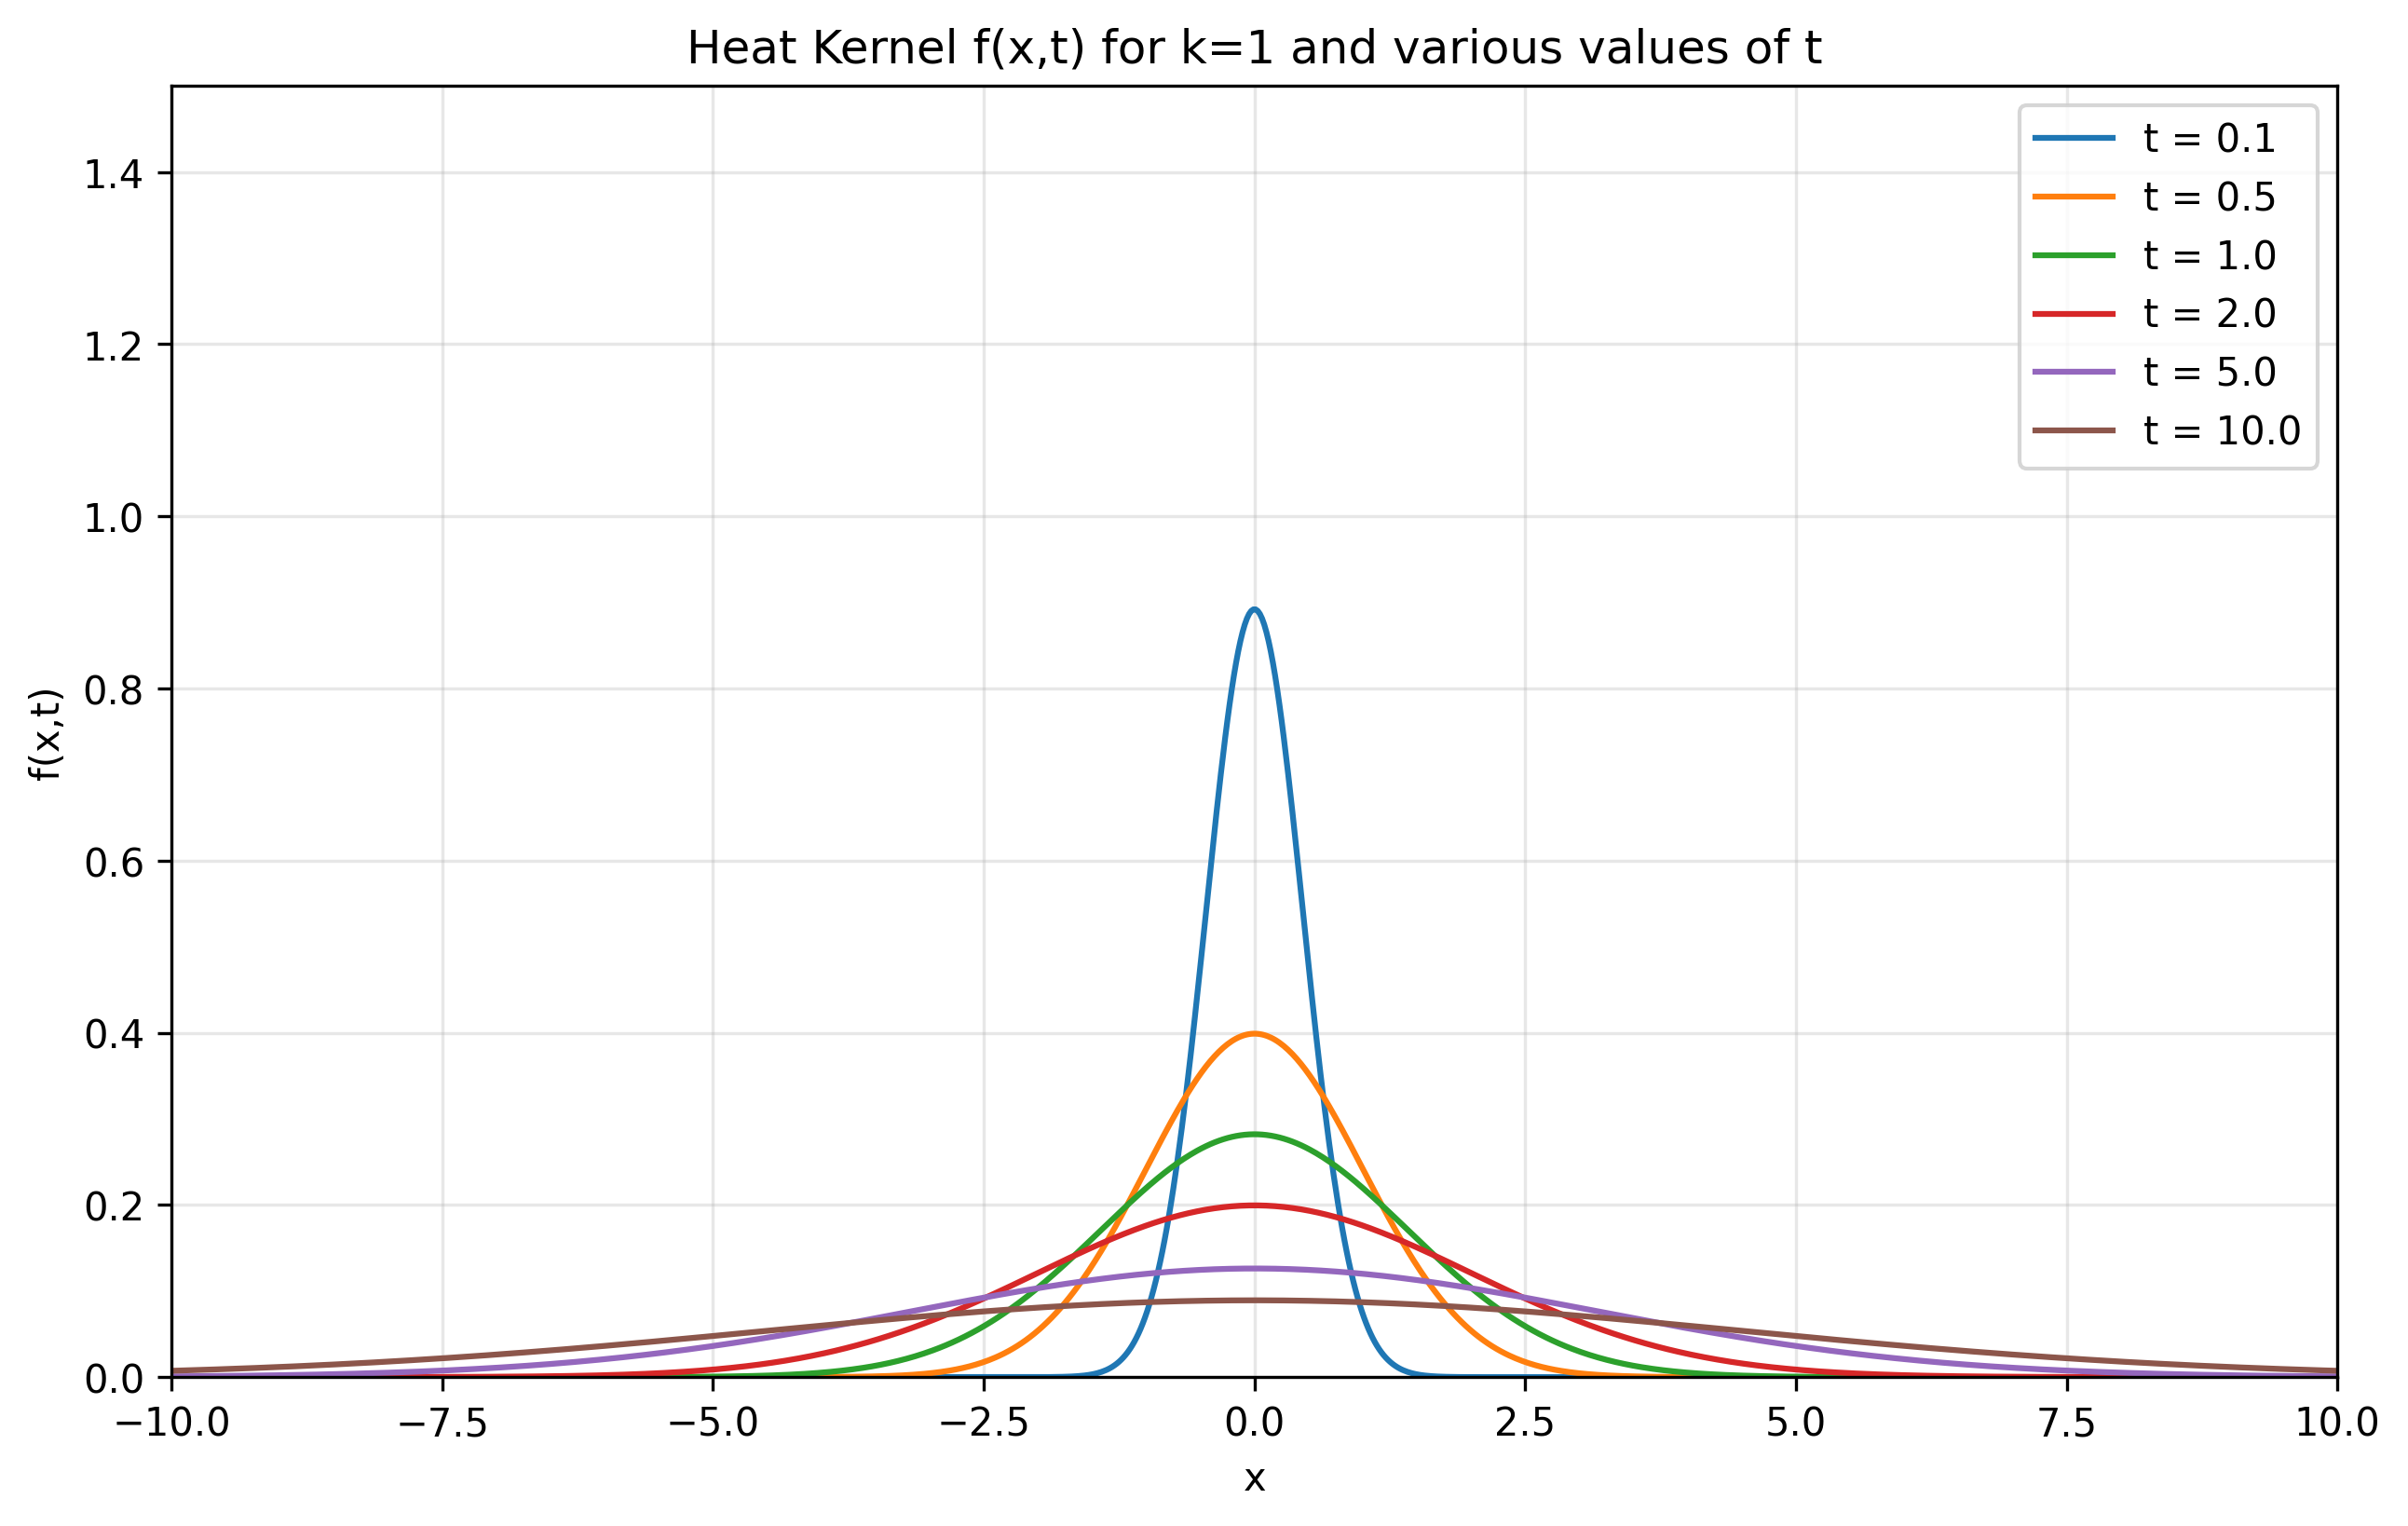
\includegraphics[width=0.8\textwidth]{heat_kernel_plot.png}
\end{center}

\textbf{Verhalten für $t \to 0$:}

Für $t \to 0$ wird die Funktion immer schmaler und höher, wobei sie sich zu einer Dirac-Delta-Distribution entwickelt:

\begin{center}
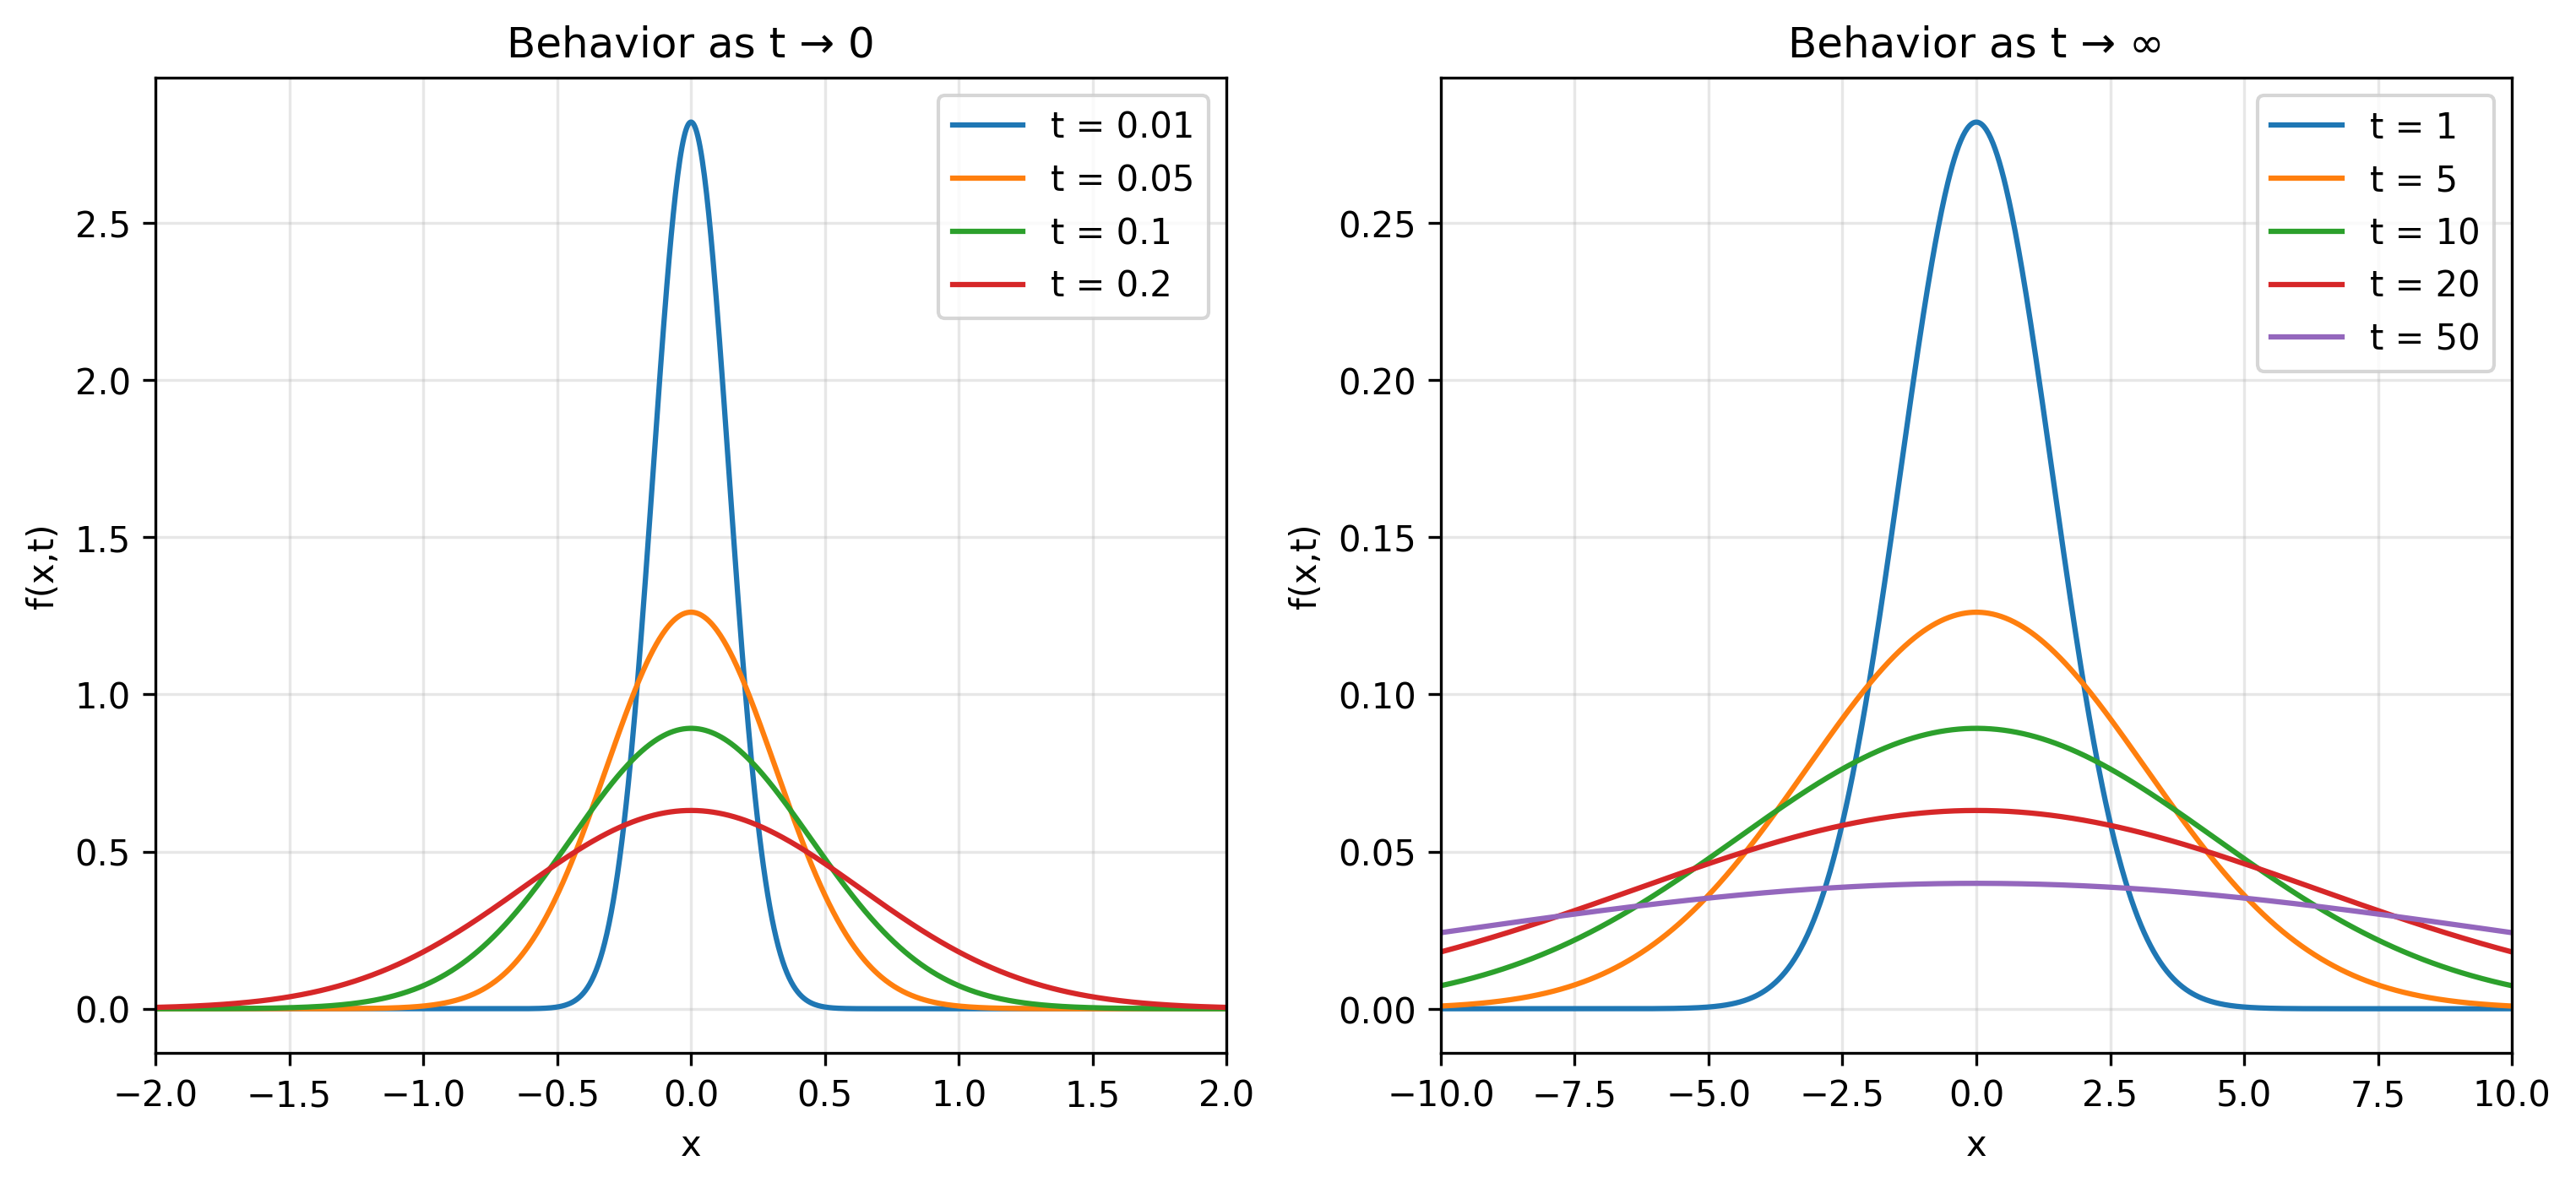
\includegraphics[width=0.8\textwidth]{heat_kernel_limits.png}
\end{center}

Mathematisch gilt:
$$\lim_{t \to 0^+} f(x,t) = \delta(x)$$

Dies bedeutet, dass für sehr kleine $t$ die gesamte ``Masse'' bei $x=0$ konzentriert ist.

\textbf{Verhalten für $t \to \infty$:}

Für $t \to \infty$ wird die Funktion immer breiter und flacher. Sie konvergiert punktweise gegen 0:
$$\lim_{t \to \infty} f(x,t) = 0 \quad \text{für alle } x \in \mathbb{R}$$

Die Standardabweichung der Verteilung ist $\sigma = \sqrt{2kt}$, was bedeutet, dass die Breite der Verteilung proportional zu $\sqrt{t}$ wächst.

\textbf{Physikalische Interpretation:}

Die Funktion $f(x,t)$ beschreibt die Wärmeverteilung in einem unendlich langen Stab, wenn zum Zeitpunkt $t=0$ die gesamte Wärmeenergie an der Stelle $x=0$ konzentriert ist (Punktquelle).

\begin{itemize}
\item Für $t \to 0$: Die Wärme ist noch nahezu vollständig am Ursprung konzentriert.
\item Für wachsendes $t$: Die Wärme breitet sich durch Diffusion aus. Die Maximaltemperatur bei $x=0$ nimmt ab, während sich die Wärme über einen immer größeren Bereich verteilt.
\item Für $t \to \infty$: Die Wärme hat sich gleichmäßig über den gesamten Stab verteilt, die Temperatur geht überall gegen 0.
\end{itemize}

Die Funktion $f(x,t)$ ist auch als \textit{Wärmekern} oder \textit{Gaußscher Kern} bekannt und spielt eine fundamentale Rolle bei der Lösung der Wärmeleitungsgleichung. Das Integral $\int_{-\infty}^{\infty} f(x,t) \, dx = 1$ bleibt für alle $t > 0$ erhalten, was der Erhaltung der Gesamtwärmeenergie entspricht.

\end{document}